\section{Complementary low-mass higgsino search}
\label{sec:ewk:LM}

The analysis discussed in this chapter is limited in sensitivity for low \mhino, as it is clear from Figure \ref{fig:exclusion_high}. 
This is because when \mhino approaches the Higgs mass, the decay products (Higgs boson and \gravino)
have increasingly low \pt, and a low \pt \gravino does not produce enough \met to satisfy the \met trigger requirements and be selected 
in the analysis. 
To gain sensitivity also to the low-\mhino part of the mass spectrum, which is particularly interesting for Naturalness arguments, 
this analysis is complemented by a second analysis that targets low-\met events, referred to as "low-mass" analysis \cite{Aaboud:2018htj}. 
Events are selected using $b$-jet triggers and are required to have at least four $b$-tagged jets, 
using a $b$-tagging \gls{op} with an efficiency of 70\%
(tighter than the 77\% used in the high-mass analysis).
This analysis uses data from 2016 where the $b$-jet triggers are available, corresponding to an integrated luminosity of 24.3 \ifb.

The jets used to reconstruct the Higgs candidates are the four with the highest $b$-tagging score, and are paired minimizing the quantity 
$D_{hh}$, defined as:
\begin{equation}
  D_{hh} = \left|m_{2j}^\textrm{lead} - \frac{120}{110}m_{2j}^\textrm{subl}\right| \; ,
\end{equation}
where $m_{2j}^\textrm{lead}$ and $m_{2j}^\textrm{subl}$ are the masses of the Higgs boson candidates with leading and subleading \pt respectively.
This pairing choice tends to create two Higgs candidates with similar mass; 
for low Higgsino masses the $b$-jets originating form the decay of the Higgs bosons are less collimated, 
and this choice is therefore more effective than minimizing \dRmax. 

The main background is constituted by multijet events and a small fraction of \ttbar events, as opposed to the
high mass analysis, where multijet is an almost-negligible background after applying the \dphimin selection. 
The background from \ttbar events is further reduced by requiring $X_{Wt}>1.8$, defined as:

\begin{equation}
 X_{Wt} = \sqrt{\left( \frac{m_W - 80.4\,\ \gev}{0.1  m_W} \right)^2 + \left( \frac{m_t - 172.5\,\ \gev}{0.1  m_t} \right)^2 } \;,
\label{eqn:xwt}
\end{equation}

\noindent where the top and W-boson candidates are built as described in Ref. \cite{Aaboud:2018htj}. 
A low value of $X_{Wt}$ corresponds to a high probability of the event to be a \ttbar event. 

The \gls{sr} is defined by requiring: 
\begin{equation}
X_{hh}^\textrm{SR} = \sqrt{ \left( \frac{m_{2j}^\textrm{lead} - 120\ \gev}{0.1 m_{2j}^\textrm{lead}} \right)^2 + \left( \frac{m_{2j}^\textrm{subl} - 110\ \gev}{0.1 m_{2j}^\textrm{subl}} \right)^2} \ <\ 1.6,
\end{equation}
\noindent where $0.1  m_{2j}^\textrm{lead}$ and $0.1 m_{2j}^\textrm{subl}$ approximate the mass resolution of the two Higgs 
boson candidates. 

The events in the \gls{sr} are further binned based on the two-dimensional distribution of \met and \meff, 
and this is used as input in the statistical analysis. The binning used is:
\begin{eqnarray*} 
\met &=& \{0, 20, 45, 70, 100, 150, 200\} \;, \\
\meffb &=&\{160, 200, 260, 340, 440, 560, 700, 860\} \;,
\end{eqnarray*}

\noindent where the values are expressed in GeV.

Two dedicated discovery regions have optimized selections to maximize the discovery significance for \mhino = 150 and 300 GeV:
\begin{description}
\item[low-SR-MET0-meff440] \meffb $>$ 440 GeV
\item[low-SR-MET150-meff440] \meffb $>$ 440 GeV, \met $>$ 150 GeV
\end{description}

The background estimate is fully data-driven and relies on a sample with exactly two $b$-tagged jets (orthogonal to the \gls{sr} and 
with very low signal contamination). $m_{2j}^\textrm{lead}$ and $m_{2j}^\textrm{subl}$ are used to define a \gls{cr} and two \glspl{vr}, both in the $\geq4b$ and in the $2b$ samples; all these regions exclude the $X_{hh}^\textrm{SR}<1.6$ area, to be orthogonal to the \gls{sr}.
The 2-tag and 4-tag \glspl{cr} are used to derive a reweighting function to go from the 2-tag sample to the 4-tag sample, that consists in two steps:
first of all an overall normalization correction is applied, and then 
a reweighting based on boosted decision trees corrects for further kinematic differences. 
This reweighting procedure is tested in the \glspl{vr} and then applied to the \glspl{vr}.
More details on the background estimate and its validation are available in Ref. \cite{Aaboud:2018htj}.

\section{Combined Results}

Figures \ref{fig:ewk:exclusion_comb} and \ref{fig:ewk:exclusion_combBR} show the combined results of the two analyses for the model-dependent 
exclusion, respectively in the case $B(\hino\rightarrow h \tilde{G})=100$\% and in the \mhino vs $B(\hino\rightarrow h \tilde{G})$ plane.
The results of the low-mass analysis are used below 300 GeV, while above it is the high-mass search that provides the nominal result.
The transition at 300 GeV is chosen such that in the transition point the two analyses have 
similar sensitivity in the case $B(\hino\rightarrow h \tilde{G})=100$\%.
In the low-mass analysis the high-\met bins of the \gls{sr} show a mild excess; 
therefore, the observed limit is weaker than expected and the portion of the mass spectrum between 230 and 290 GeV is not excluded in the 
$B(\hino\rightarrow h \tilde{G})=100$\%, despite the expected sensitivity. 

\begin{figure}[htbp]
	\centering
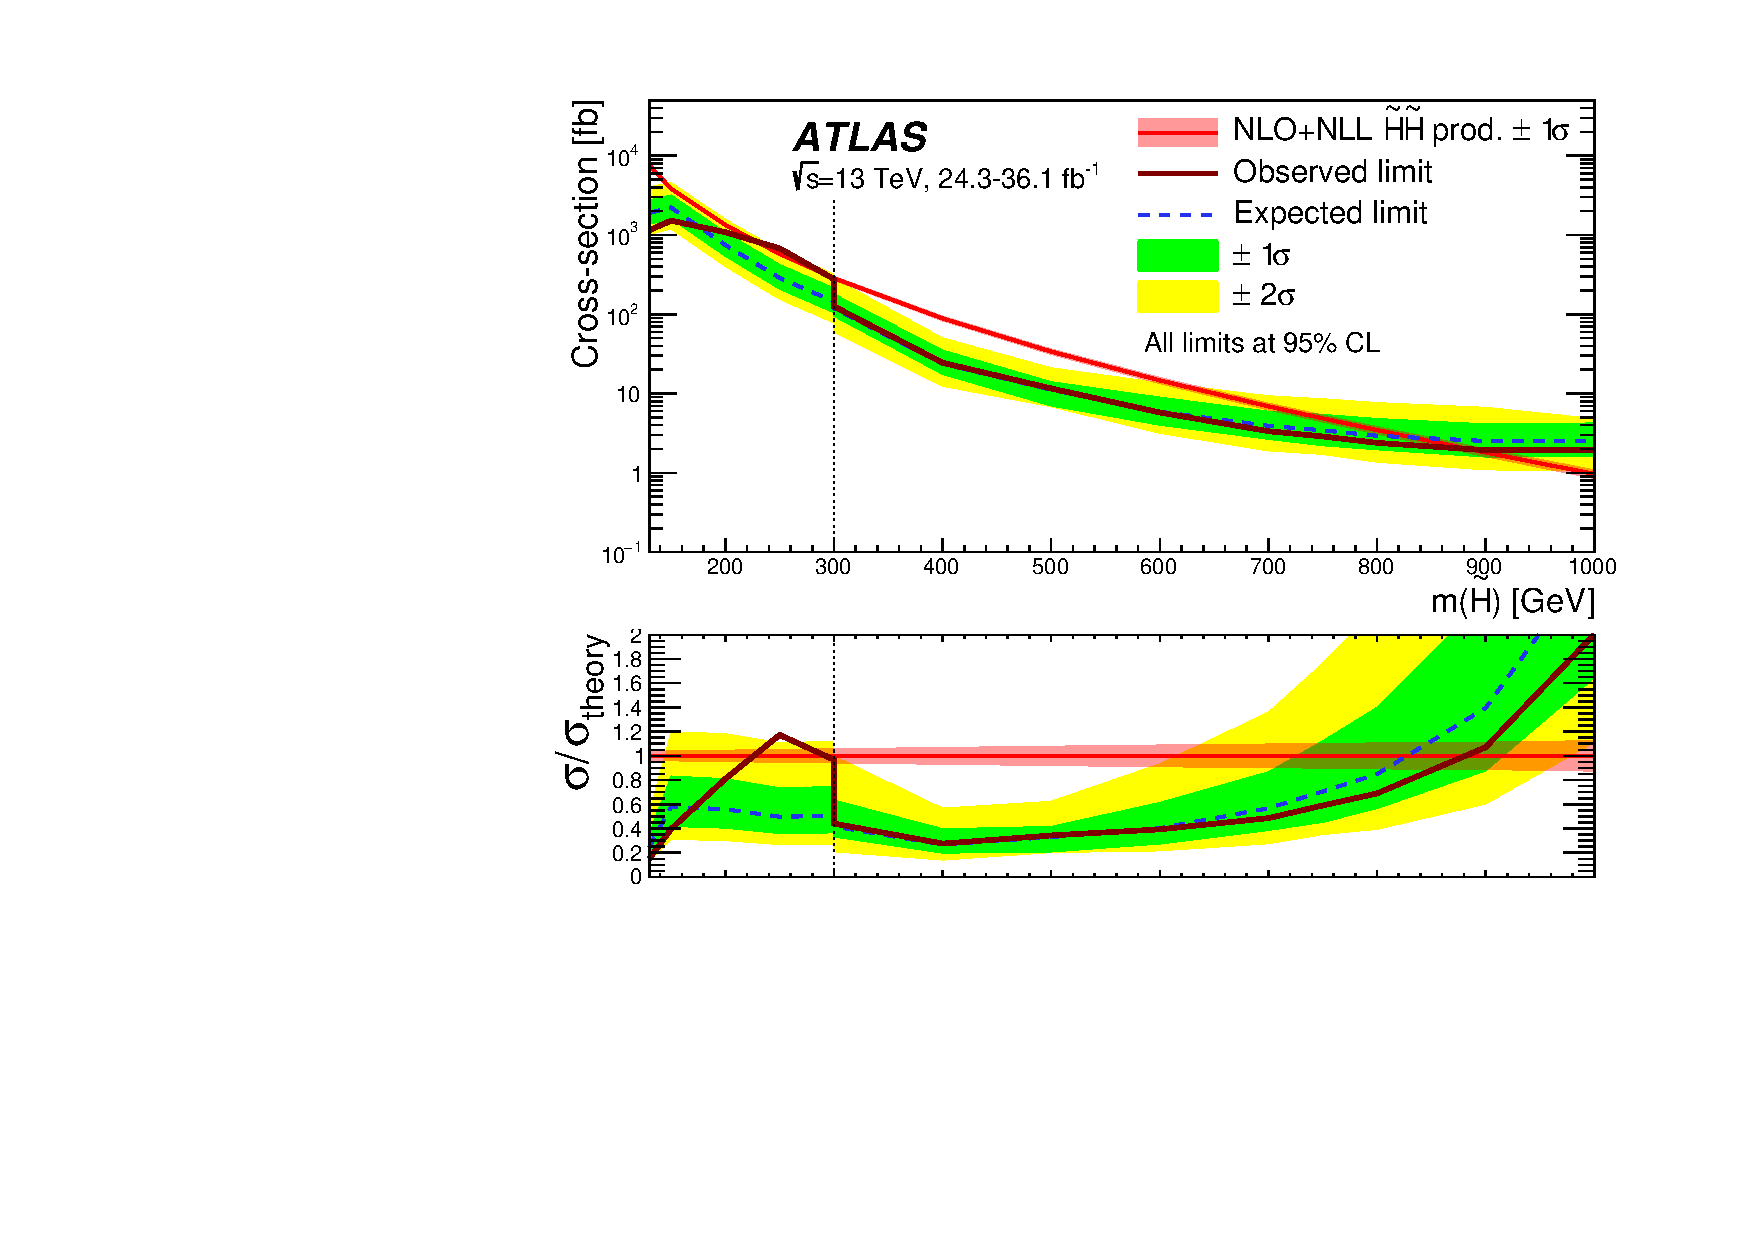
\includegraphics[width=0.75\textwidth]{figures/ewk_prod/interpretation/GGMupperLimit_unblinded_jump}
	\caption{The observed (solid) vs expected (dashed) 95\% upper limits on the \hino\ pair production cross-section as a function of \mhino.  The 1$\sigma$ and 2$\sigma$ uncertainty bands on the expected limit are shown as green and yellow, respectively. The theory cross-section and its uncertainty are shown in the solid and shaded red curve.
   The results of the low-mass analysis are used below $\mhino = 300$ GeV, while those of the high-mass analysis are used above. 
   Figure from Ref. \cite{Aaboud:2018htj}. } 
	\label{fig:ewk:exclusion_comb}
\end{figure}


\begin{figure}[htbp]    
	\centering    
    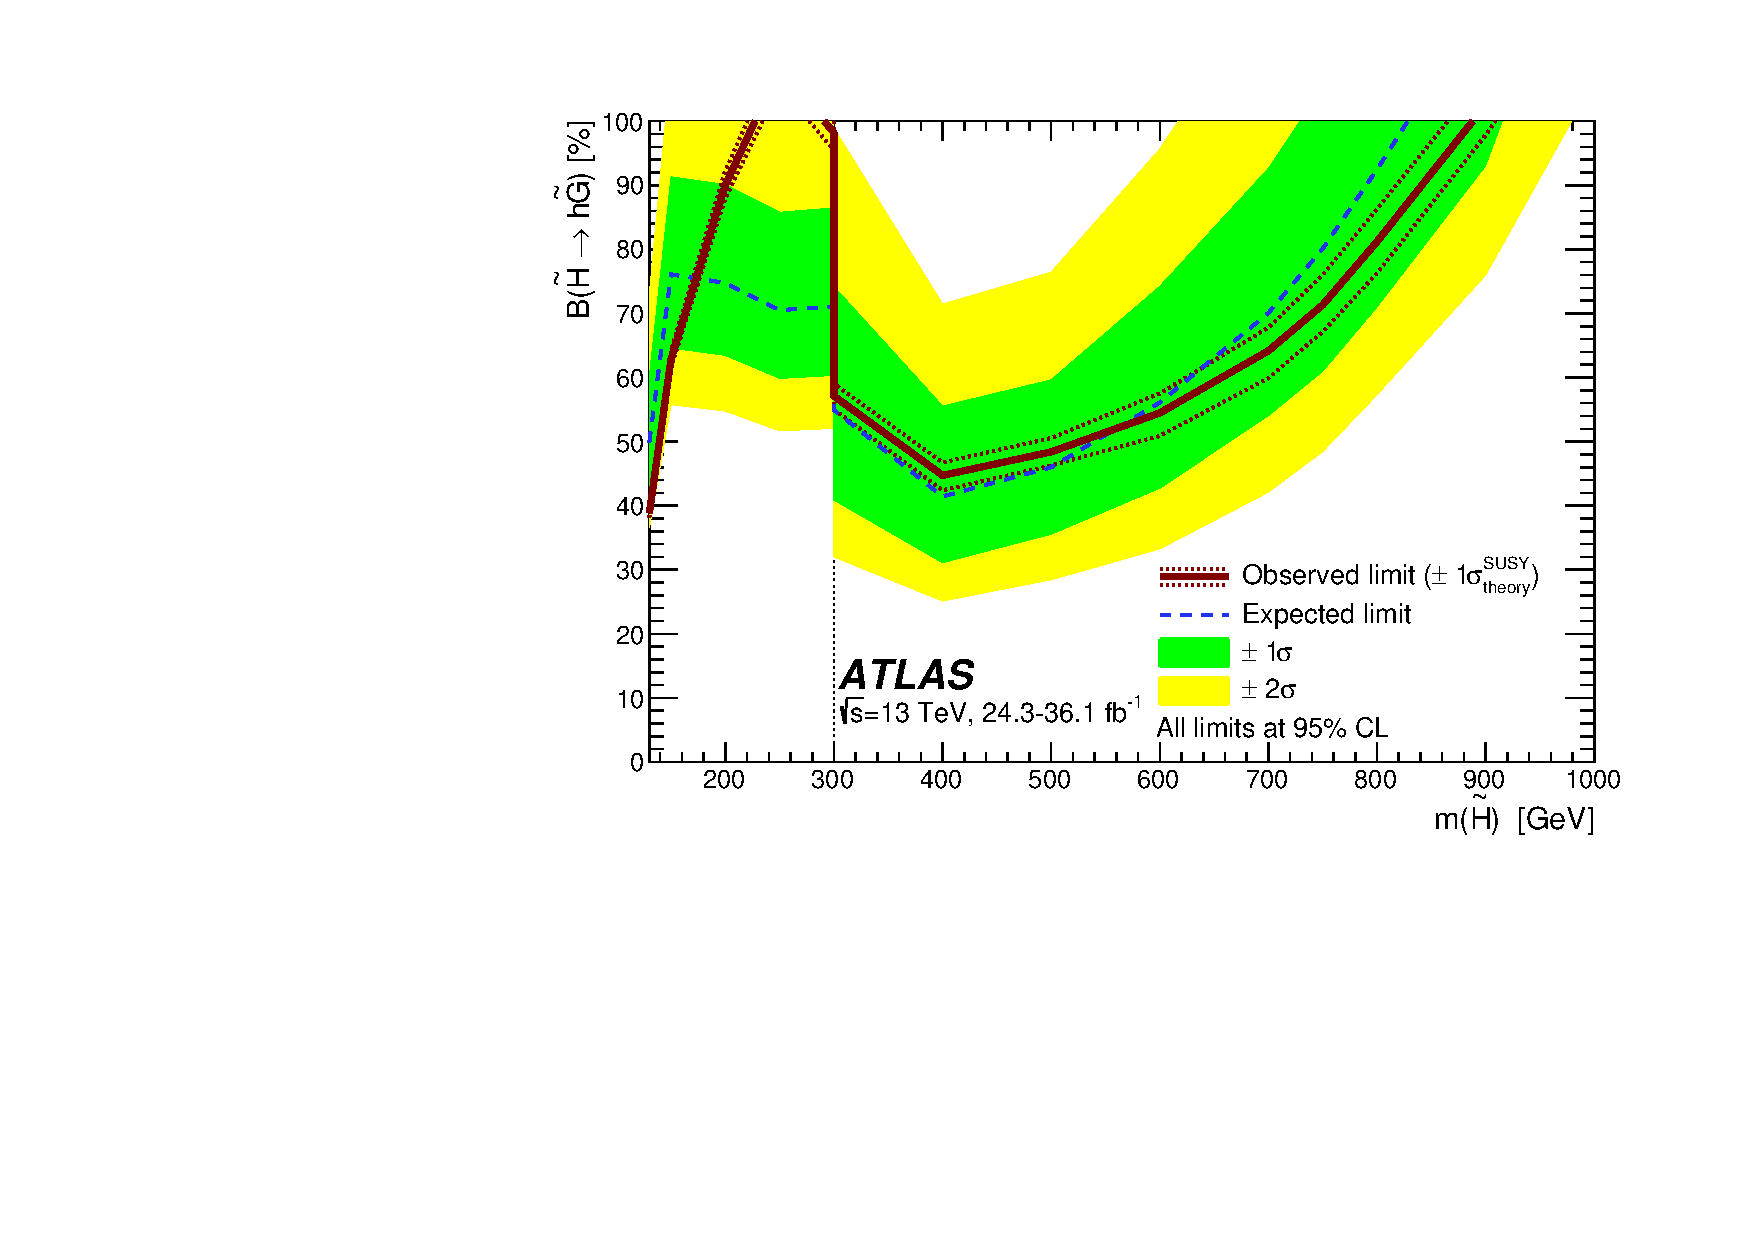
\includegraphics[width=0.75\textwidth]{figures/ewk_prod/interpretation/my_br_plot_unblind_yellow_band}\label{fig:exclusion_br}
	\caption{The observed (solid) vs expected (dashed) 95\% limits in the \mhino\ vs $B(\hino\rightarrow h \tilde{G})$ plane, where $B(\hino\rightarrow h \tilde{G})$ denotes the branching ratio for the decay $\hino \rightarrow h \gravino$. The 1$\sigma$ uncertainty band is overlaid in green and the 2$\sigma$ in yellow.
	The results of the low-mass analysis are used below $\mhino = 300$ GeV, while those of the high-mass analysis are used above.
	 The regions above the lines are excluded by the analyses. Figure from Ref. \cite{Aaboud:2018htj}. } 
	\label{fig:ewk:exclusion_combBR}
\end{figure}


